\section{AES}
The first cryptography scheme we attempted to accelerate was AES, a symmetric key cryptography algorithm. AES is primarily used as a block cipher, which has openly exploitable parallelism by encrypting multiple blocks at once. Thus we saw AES as a prime candidate to optimize with hardware for large amounts of data. The AES implementation was based off of the NIST documentation\footnote{NIST guide to AES: \url{https://nvlpubs.nist.gov/nistpubs/FIPS/NIST.FIPS.197.pdf}.} on AES as well as the github library tiny-AES-c\footnote{Embedded optimized tiny-AES-c library: \url{https://github.com/kokke/tiny-AES-c}.}. While it would be nice to make a hardware implementation that can beat a modern day computer, it is unlikely due to how many Watts are pushed to modern day CPUs. Thus our evaluation will be done comparing the smaller zedboards primarily against microprossers, such as the zedboard's built in ARM chip. 

\subsection{Techniques}
% This section should provide a detailed description of the applications, algorithms, or
% hardware architectures realized in this project. Think critically about the important items to mention
% in order for the reader to understand how your design works without having to look into any code.
% For example, what are the inputs and outputs of the application (or architecture), what are the major
% steps (or modules), and what does each step (or module) achieve? It would be useful to include
% small examples, block diagrams, mathematical formulas, and other visualizations to help explain your
% techniques. Do not include detailed information about your source code as your report should be at a
% high level.
The AES algorithm is a fairly simple one, consisting of a number of rounds operating on a 4x4 byte matrix state to encrypt the 16-byte buffer input using a key. The key size can be configured as 128, 192, or 256 bits wide. The larger the key, the more rounds that run on the state. Each round consists of four main operations called AddRoundKey, SubBytes, ShiftRows, and MixColumns. Before all of this begins, the key needs to be expanded into a key schedule, called a RoundKey, which a portion of it is XOR'd with the state each round during AddRoundKey. SubBytes is a one-to-one substitution of each byte value in the state, which is done using an Sbox, generated using finite field arithmatic, which is beyond the scope of this paper. ShiftRows is a simple rotation of rows in the matrix by differing offsets. Lastly, MixColumns operates on the columns of the state, performing some matrix multiplication with each column, but also doing things with the Galois Field that are beyond the scope of this paper as well.  

In order to exploit the most parallelism from the algorithm, we want to be able to pipeline these rounds such that we can be performing AES on multiple blocks as a time without duplicating hardware. AES ECB allows us to do that, but it is also very insecure and thus no one practically uses this on large amounts of information. AES CBC is not great for parallelism because in order to start the next block, it first must be XOR'd with the encrypted previous block. Thus we selected the AES CTR method, which uses a nonce/IV and a counter, encryptes the counter value and XORs that with the plaintext. This allows us to pipeline the encryption easily as each value being encrypted is one plus the previous value. Figure \ref{fig:aesctr} shows with a diagram how AES CTR works, taking in 16-byte blocks and encrypting them with AES. 

\begin{figure}[h]
\centering
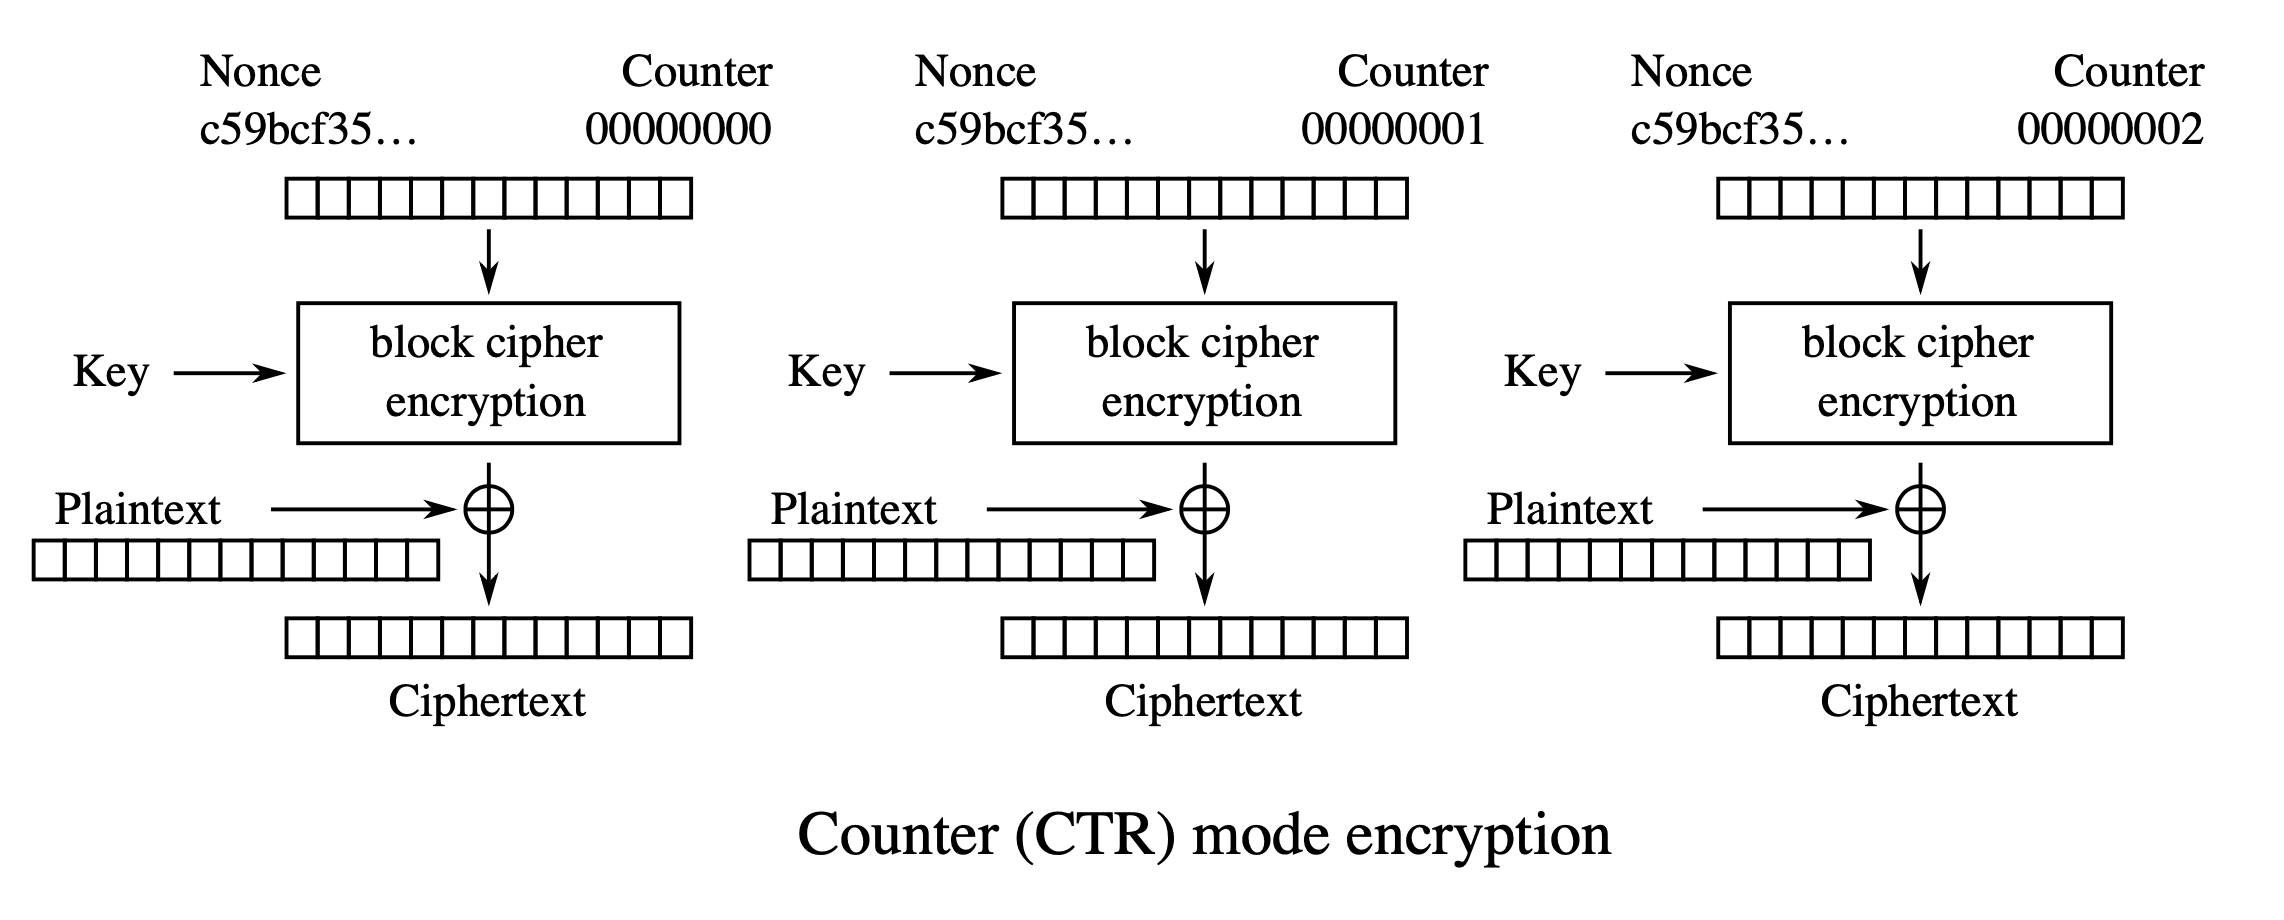
\includegraphics[width=0.5\textwidth]{aesctr}
\caption{AES CTR diagram.}
\label{fig:aesctr}
\end{figure}

\subsection{Implementation}
% This section describe how you implemented your designs. For example, what
% programming languages did you use? Did you take advantage of any third-party libraries? Is your
% implementation purely software, purely hardware, or a mix of both? Which software and/or hardware
% blocks are included in your design, and what hardware device (if any) did you target? In most cases, it
% would be helpful to include block diagrams of your implementation illustrating the flow of data through
% your design, the interconnection between different blocks, and whether each block is implemented
% in software or hardware. As in the previous section, providing meaningful visualizations would help
% the reader better appreciate your work. Please also include one or two interesting aspects of your
% implementation, especially any specific implementation strategies necessary for creating a functionally
% correct design with good performance.
Our optimizied hardware synthesizable version was built using C++ and the Vivado ap\_int library. Our goal was to synthesize AES for the small zedboard and compete against the zedboard ARM CPU. Normally AES is implemented by taking a 16-byte array and converting that into a 4x4 byte matrix as the state, storing the bytes incrementing column-wise as in Figure \ref{fig:aesstate}. We, however, pack the 16-byte block into one 128-bit number, which is simple as well because we can place the bytes starting in the least significant bits of the number. The key is also stored as an X-bit number, where the X is determined by the key length. The RoundKey we pack into 128-bit numbers, and store as an array of 128-bit values, one for each round. This is extremely helpful, as the AddRoundKey function just becomes one XOR with the current round's key schedule. The other functions (except ShiftRows), contain loops to loop over each byte or each column. These we completely unroll, as they can all be done in parallel, and it actually reduces area because indexing into the large ap\_uints variably was more expensive than direct wires connected to the bits of the state. ShiftRows was already just a bunch of wire rearrangements and required no optimization. In the end, the four main functions had 0 or 1 cycle latencies, the 1 cycle for indexing into the Sbox or the RoundKey arrays. Ideally we could fully partition those, and reduce those latencies to just combinational logic, but this took too much area. 

\begin{figure}[h]
\centering
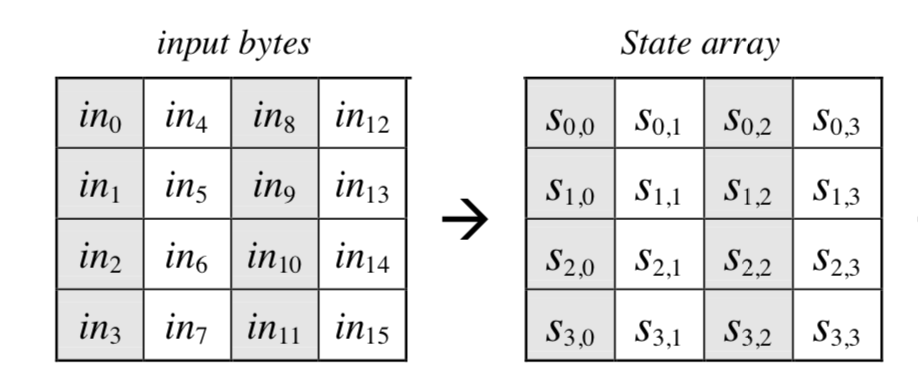
\includegraphics[width=0.5\textwidth]{aesstate}
\caption{AES CTR diagram.}
\label{fig:aesstate}
\end{figure}

In our top level, we have a loop that reads in values, ciphers the counter, XORs to get the plaintext and writes this value out. We pipeline this loop, as the Cipher function is inlined. This ideally pipelines our rounds as well, allowing us to read data and then pushing it through as the next block for AES.  

\subsection{Evaluation}
% Students should describe the experimental setup used to evaluate their design. Students
% should describe the data inputs used to evaluate their design and provide an analysis of the achieved
% results. The results should be clearly summarized in terms of tables, text, and/or plots. Please provide
% qualitative and quantitative analysis of the results and discuss insights from these results. Results may
% include (but are not limited to) the execution time of an algorithm, hardware resource usage, achievable
% throughput, and error rate. It would be interesting, for example, to discuss why one design is better
% than another, why one design achieves a higher metric than another, or how you trade-off one metric
% for another. Consider going into detail for one particular instance of your experiment and analyze how
% it achieves the given results.
In order to evaluate our optimized FPGA version, we create a host program that reads 8000 bytes of data, sends the key, initiation vector, and data to the FPGA, and then reads back the encrypting data and compares that to the pre-saved encrypted data for testing. Based on our synthesize report, our pipelined block loop had an II of 4 and a depth of 46. Thus we deemed 500 blocks sufficient for measuring speedup as we have well surpassed the warm up and cool down times of the pipeline. The final area usage was drastically lower than expecting, reaching only about 37\% of the LUTs. The full area usage for AES-256 is in Table \ref{table:aesarea}. 

\begin{table}[h]
\begin{center}
\begin{tabular}{| c | c | c | c | c |}\hline
& BRAM\_18K &  DSP48E &   FF    &  LUT \\\hline
Utilization (\%)  &       15 &      0 &       6 &     37 \\\hline
\end{tabular}
\label{table:aesarea}
\caption{The final area usage of AES-256 (other key-lengths are very similar).}
\end{center}
\end{table}

For a final comparison, we passed the same 8000 bytes through the tiny-AES-c embedded processor optimized version of AES on both the ecelinux server's as well as the zedboard's microprocessor. The results of this test along with the FPGA baseline, FPGA optimized, and ecelinux optimized csim times are in Table \ref{table:aestime}. As we can see, both ecelinux runs beat the FPGA by an order of magnitude, which is largely expected. The FPGA does successfully beat the Zedboard's ARM processor, with a resulting speedup of about 1.75x. The FPGA baseline times are estimated because they wouldn't actually synthesize due to too much area usage. We believe this is because without unrolling some loops, the variable slicing of the large ap\_uints require a lot of muxing, thus producing much more area. 

\begin{table}[h]
\begin{center}
\begin{tabular}{| c | c | c | c |}\hline
Test & AES128 (ms) & AES192 (ms) & AES256 (ms) \\\hline
ecelinux-sw & 1.6 & 1.9 & 2.1 \\\hline
ecelinux-csim & 5.1 & 6.2 & 7.2 \\\hline
zedboard-sw & 25.5 & 30.0 & 34.3 \\\hline
fpga-baseline & 4560 & 5820 & 4120 \\\hline
fpga-opt & 19.3 & 20.5 & 17.5 \\\hline
\end{tabular}
\label{table:aestime}
\caption{The results of the tests run for evaluation.}
\end{center}
\end{table}

Overall, these results bode well for a hardware implementation of AES. In embedded scenarios where fast AES is needed for large amounts of data, the FPGA could be extremely useful. The Zedboard's only use about 5 Watts in comparison to ecelinux which can burn hundreds of Watts. Another thing to consider is as we send more data, the bandwith required to read and send this data will increase, and could cause slowdowns there. In a situation where an embedded processor is used, and power is a major constraint, using the FPGA could be a viable option as it provides a speedup while keeping power usage down at the expense of more area. 